\documentclass{article} % For LaTeX2e
\usepackage{nips15submit_e,times}
\usepackage{hyperref}
\usepackage{url}
\usepackage{graphicx}
\usepackage{float}
\usepackage{amsmath}
\usepackage{multirow,array}
\usepackage{listings}
\usepackage{amsfonts}
\usepackage{caption}
\usepackage{subfigure}
\usepackage{algorithm,algorithmic}
%\usepackage[UTF8]{ctex} uncomment if needs Chinese support
%\usepackage{fontspec}

%\documentstyle[nips14submit_09,times,art10]{article} % For LaTeX 2.09

\renewcommand{\algorithmicrequire}{ \textbf{Input:}} %Use Input in the format of Algorithm
\renewcommand{\algorithmicensure}{ \textbf{Output:}} %UseOutput in the format of Algorithm

\definecolor{mygreen}{rgb}{0,0.6,0}
\definecolor{mygray}{rgb}{0.5,0.5,0.5}
\definecolor{mymauve}{rgb}{0.58,0,0.82}
\lstset{ %
backgroundcolor=\color{white},   % choose the background color
basicstyle=\footnotesize\ttfamily,        % size of fonts used for the code
columns=fullflexible,
breaklines=true,                 % automatic line breaking only at whitespace
captionpos=b,                    % sets the caption-position to bottom
tabsize=4,
commentstyle=\color{mygreen},    % comment style
escapeinside={\%*}{*)},          % if you want to add LaTeX within your code
keywordstyle=\color{blue},       % keyword style
stringstyle=\color{mymauve}\ttfamily,     % string literal style
frame=single,
rulesepcolor=\color{red!20!green!20!blue!20},
% identifierstyle=\color{red},
language=python,
numbers=left
}

\title{Weekly Report(May 14 - May 20)}


\author{
Liu Junnan
}

% The \author macro works with any number of authors. There are two commands
% used to separate the names and addresses of multiple authors: \And and \AND.
%
% Using \And between authors leaves it to \LaTeX{} to determine where to break
% the lines. Using \AND forces a linebreak at that point. So, if \LaTeX{}
% puts 3 of 4 authors names on the first line, and the last on the second
% line, try using \AND instead of \And before the third author name.

\newcommand{\fix}{\marginpar{FIX}}
\newcommand{\new}{\marginpar{NEW}}

%\nipsfinalcopy % Uncomment for camera-ready version

\begin{document}
	
\maketitle

\begin{abstract}
This week I finished assignment2 including the implementation of convolutional layer and \{batch, layer, spatial batch, group\}normalization layers, plus pytorch version of convnets. This report covers the details in the implementation of these topic mentioned above. 
\end{abstract}

\section{Work Done}
\subsection{Convolutional Layer - Implementation}
Recall that a convolutional layer consists of several filters that convolves input images and produces a feature map.
\begin{figure}[H]
	\centering
	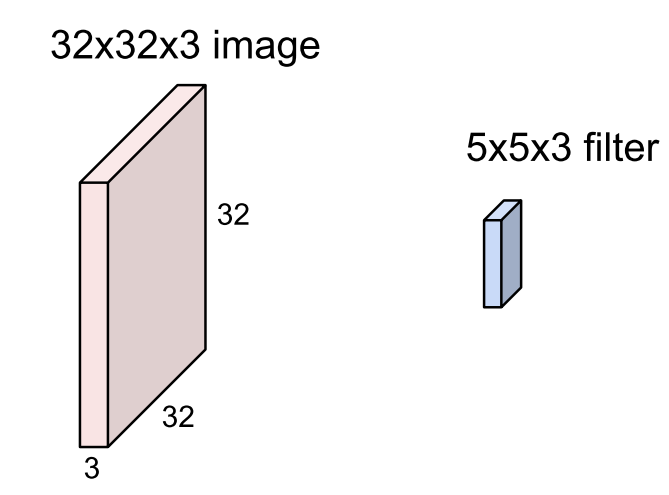
\includegraphics[width=.5\textwidth]{convlayer.png}
	\caption{Convolutional Layer Example}
\end{figure}

Specifically, $x$ is input data of shape $(N, C, H, W)$, where $N$ is the mini-batch size, $C$ number of channels, $H$ and $W$ are height and width of each channel; $w$ is filter weights of shape $(F, C, HH, WW)$ where $F$ is the number of filters, $HH$ and $WW$ are height and width of a filter. Then we can compute the shape of output by the formulation mentioned in the previous report:

\begin{eqnarray*}
H' &=& \frac{1 + (H + 2 * \text{pad} - HH)}{\text{stride}}\\
W' &=& \frac{1 + (W + 2 * \text{pad} - WW)}{\text{stride}}
\end{eqnarray*}

The naive version of forward pass of conv layer with 4 loops is as follows:
\begin{lstlisting}
Ho = 1 + (H + 2 * pad - HH) // stride
Wo = 1 + (W + 2 * pad - WW) // stride

x_pad = np.pad(x, ((0, 0), (0, 0), (pad, pad), (pad,pad)), 'constant')
out = np.zeros((N, F, Ho, Wo))

for n in range(N):
	for i in range(Ho):
		for j in range(Wo):
			for k in range(F):
				out[n, k, i, j] = np.sum(
				x_pad[n, :, i*stride:i*stride+HH, j*stride:j*stride+WW] * w[k]) + b[k]
\end{lstlisting}
It computes element-wise multiplication of blocks of input data and filter matrices over channels and batch samples. 

A simple modification could help the code vectorized
\begin{lstlisting}
for i in range(Ho):
	for j in range(Wo):
		x_pad_masked = x_pad[:, :, i*stride: i*stride+HH, j*stride: j*stride+WW]
		mul = x_pad_masked.reshape((N, -1, C, HH, WW)) * w.reshape((-1, F, C, HH, WW))
		out[:, :, i, j] = np.sum(mul, axis=(2, 3, 4))
out += b.reshape((1, F, 1, 1))
\end{lstlisting}

However, the backward pass of conv layer is quite tricky and it is not detailed in the cs231 course. This part is based on a blog on the Internet since it's quite mathematically difficult to derive. Recall that the forward activation of a convolutional layer is computed by
$$a^l=\sigma(z^l)=\sigma(a^{l-1}*W^l + b^l)$$
where the superscripts mean the variables in the $l$-th layer respectively, and $\sigma$ denotes the activation function, $z$ the input and $a$ the activation/output value.

Then we can compute the gradient of $l$-th layer by
$$\delta^{l-1}=\frac{\partial J(W,b)}{\partial z^{l-1}}=\frac{\partial J(W,b)}{\partial z^{l}} \frac{\partial z^l}{\partial z^{l-1}}=\delta^l \frac{\partial z^l}{\partial z^{l-1
}}$$
\begin{eqnarray}
z^l = a^{l-1}*W^l +b^l
\label{eqn:1}
\end{eqnarray}

We can simplify the setting that, say, $a$ is a $3 \times 3$ matrix, $w$ is a $2 \times 2$ matrix, and $b$ is a zero matrix. Then eqn\ref{eqn:1} can be written as

\begin{eqnarray}
\left( \begin{array}{ccc} 
	a_{11}&a_{12}&a_{13} \\ 
	a_{21}&a_{22}&a_{23}\\ 
	a_{31}&a_{32}&a_{33} 
	\end{array} \right)    
*  
\left( \begin{array}{ccc} 
	w_{11}&w_{12}\\ 
	w_{21}&w_{22} 
\end{array} \right) 
=
\left( \begin{array}{ccc} 
	z_{11}&z_{12}\\ 
	z_{21}&z_{22} 
\end{array} \right)
\label{eqn:2}
\end{eqnarray}

Stretch the convolution in eqn\ref{eqn:2} as
\begin{eqnarray}
z_{11} &=& a_{11}w_{11} + a_{12}w_{12} + a_{21}w_{21} +   a_{22}w_{22}\\
z_{12} &=& a_{12}w_{11} + a_{13}w_{12} + a_{22}w_{21} +   a_{23}w_{22}\\
z_{21} &=& a_{21}w_{11} + a_{22}w_{12} + a_{31}w_{21} +   a_{32}w_{22}\\
z_{22} &=& a_{22}w_{11} + a_{23}w_{12} + a_{32}w_{21} +   a_{33}w_{22}
\end{eqnarray}

The gradient with respect to $a^{l-1}$ is
$$\nabla a^{l-1} = \frac{\partial J(W,b)}{\partial a^{l-1}} = \frac{\partial J(W,b)}{\partial z^{l}} \frac{\partial z^{l}}{\partial a^{l-1}} = \delta^{l} \frac{\partial z^{l}}{\partial a^{l-1}}$$

Then we can compute $\frac{\partial z^{l}}{\partial a^{l-1}}$ element-wise:

\begin{eqnarray*}
\nabla a_{11} &=& \delta_{11}w_{11}\\
\nabla a_{11} &=& \delta_{11}w_{11}\\
\nabla a_{11} &=& \delta_{11}w_{11}\\
\nabla a_{21} &=& \delta_{11}w_{21} + \delta_{21}w_{11}\\
\nabla a_{22} &=& \delta_{11}w_{22} + \delta_{12}w_{21} + \delta_{21}w_{12} + \delta_{22}w_{11}\\
\nabla a_{23} &=& \delta_{12}w_{22} + \delta_{22}w_{12}\\
\nabla a_{31} &=& \delta_{21}w_{21}\\
\nabla a_{32} &=& \delta_{21}w_{22} + \delta_{22}w_{21}\\
\nabla a_{33} &=& \delta_{22}w_{22}
\end{eqnarray*}

Actually these equations can be represented as a convolution operation:
\begin{eqnarray*}
	\left( \begin{array}{cccc} 
		0&0&0&0 \\ 
		0&\delta_{11}& \delta_{12}&0 \\ 
		0&\delta_{21}&\delta_{22}&0 \\ 
		0&0&0&0 \end{array} \right) 
	* 
	\left( \begin{array}{ccc} 
		w_{22}&w_{21}\\ 
		w_{12}&w_{11} 
	\end{array} \right)  
	= 
	\left( \begin{array}{ccc} 
		\nabla a_{11}&\nabla a_{12}&\nabla a_{13} \\ 
		\nabla a_{21}&\nabla a_{22}&\nabla a_{23}\\ 
		\nabla a_{31}&\nabla a_{32}&\nabla a_{33} 
	\end{array} \right)
\end{eqnarray*}

Notice that $\left( \begin{array}{ccc} 
w_{22}&w_{21}\\ 
w_{12}&w_{11} 
\end{array} \right)  = rot180(W)$

In summary, $\nabla a^{l-1}=\sigma^l * rot180(W^l)$

Similarly, 
$$\nabla W^{l} = \frac{\partial J(W,b)}{\partial z^{l}}\frac{\partial z^{l}}{\partial W^{l}} =\delta^l*rot180(a^{l-1})$$
and
$$\frac{\partial J(W,b)}{\partial b^{l}} = \sum\limits_{u,v}(\delta^l)_{u,v}$$

The formulations above still seem difficult to understand. But the intuition is that because of the weight sharing mechanism of convolution networks, each block of input data(of shape $(HH,WW)$, i.e. the filter size) connects to a "replica" of the same filter and do element-wise multiplication in the forward pass. So in backward pass, you only have to compute the individual gradient for each block and replica, and sum over the gradients of replicas as the final gradient with respect to that filter.

The code is as follows:
\begin{lstlisting}
padding = [(0,0), (0, 0), (pad, pad), (pad, pad)]
x_pad = np.pad(x, padding, 'constant')
dout_pad = np.pad(dout, padding, 'constant')

db = np.sum(dout, axis=(0,2,3))
for i in range(Ho):
	for j in range(Wo):
		x_pad_masked = x_pad[:, :, i*stride:i*stride+HH, j*stride:j*stride+WW]
		for k in range(F):
			dw[k] += np.sum(x_pad_masked * (dout[:, k, i, j])[:, None, None, None], axis=0)
		for n in range(N):
			dx_pad[n, :, i*stride:i*stride+HH, j*stride:j*stride+WW] +=\
				np.sum(w*(dout[n, :, i, j])[:, None, None, None], axis=0)

dx = dx_pad[:, :, pad:-pad, pad:-pad]
\end{lstlisting}
We do padding is due to the shape issue. In each element of the feature map/output(code line 6-8) we extract the responsible block of input x, and use it to compute gradient. Line 15 removes the padded area of dx.

Again, backpropagation of conv layer is quite tricky. Even though I referred to many blogs and materials, I still don't think I fully understand the math behind it. But at least I can implement the code if the formulations are given. 

\subsection{Normalization Layers - Implementation}
I have already finished the naive version of batch normalization layer last week, but still remains improvement to do. Besides there are still several variants like layer normalization, spatial batch normalization and spatial group normalization.

\subsubsection{Batch Normalization}
Recall that batch normalization can be computed by the following equations:
Forward:
\begin{eqnarray*}
	\mu &=& \frac{1}{m} \sum_i x_i\\
	\sigma^2 &=& \frac{1}{m}\sum_i (x_i-\mu)^2\\
	\hat{x_i} &=& \frac{x_i-\mu}{\sqrt{\sigma^2+\epsilon}}\\
	y_i &=& \gamma \hat{x_i} + \beta
\end{eqnarray*}
Backward:
\begin{eqnarray*}
	\nabla \hat{x_i} &=& \gamma \cdot \nabla y_i\\
	\nabla \sigma^2 &=& \sum_j \nabla \hat{x_i} \cdot (x_j - \mu) \cdot \frac{-1}{2} (\sigma^2 + \epsilon)^{-\frac{3}{2}}\\
	\nabla \mu &=& \left(\sum_i \nabla \hat{x_i} \cdot \frac{-1}{\sqrt{\sigma^2+\epsilon}}\right) + \nabla{\sigma^2} \frac{\sum_i -2(x_i-\mu)}{m}\\
	\nabla x_i &=& \nabla \hat{x_i} \cdot \frac{1}{\sqrt{\sigma^2 + \epsilon}} + \nabla \sigma^2 \cdot \frac{2(x_i-\mu)}{m} + \frac{\nabla{\mu}}{m}\\
	\nabla \gamma &=& \sum_i \nabla y_i \cdot \hat{x_i}\\
	\nabla \beta &=& \sum_i \nabla y_i
\end{eqnarray*}

Following the above equations step by step we can write the naive version of batch normalization:
\begin{lstlisting}
m = x_hat.shape[0]

dx_hat = dout * gamma
dvar_inner = dx_hat * (x - sample_mean) * var_inv**3
dvar = -0.5 * np.sum(dvar_inner, axis=0)
dmean = -np.sum(dx_hat * var_inv, axis=0) + -2 * dvar * np.mean(x - sample_mean, axis=0)
dx = dx_hat * var_inv + 2 / m * dvar * (x - sample_mean) + dmean / m
dgamma = np.sum(x_hat*dout, axis=0)
dbeta = np.sum(dout, axis=0)
\end{lstlisting}
where variable $var$ means $\sigma^2$, and $var\_inv$ stands for $\frac{1}{\sqrt{\sigma^2+\epsilon}}$ for simplification.

Actually the computation of intermediate variables $\nabla \mu$ and $\nabla \sigma^2$ is unnecessary and code line 4-7 can be re-written in one line of less than 80 characters if spaces are omitted, which is the requirement of the assignment.

\begin{eqnarray*}
\nabla \sigma^2 &=& \sum_i \nabla \hat{x_i} \cdot (x_i - \mu) \cdot \frac{-1}{2} (\sigma^2 + \epsilon)^{-\frac{3}{2}} = -\frac{1}{2} \cdot \sum_i \nabla \hat{x_i} \frac{x_i-\mu}{\sqrt{\sigma^2+\epsilon}} \cdot \frac{1}{\sqrt{\sigma^2+\epsilon}}\\
&=& -\frac{1}{2(\sigma^2+\epsilon)} \sum_i \nabla \hat{x_i} \hat{x_i}
\end{eqnarray*}

\begin{eqnarray*}
\nabla \mu &=& \left(\sum_i \nabla \hat{x_i} \cdot \frac{-1}{\sqrt{\sigma^2+\epsilon}}\right) + \nabla{\sigma^2} \frac{\sum_i -2(x_i-\mu)}{m}
\end{eqnarray*}
In the above equation
$$\sum_i x_i - \mu = \sum_i x_i - \sum_i \mu =m*\mu - m * \mu=0$$
Therefore $\nabla \mu = \frac{-1}{\sqrt{\sigma^2+\epsilon}} \cdot \sum_i \nabla \hat{x_i}$

Assemble them together we can get $\nabla \hat{x_i}$ as:
\begin{eqnarray*}
	\nabla \hat{x_i} &=& \left(\nabla \hat{x_i} \cdot \frac{1}{\sqrt{\sigma^2 + \epsilon}}\right) + \left(\nabla \sigma^2 \cdot \frac{2(x_i-\mu)}{m}\right) + \left(\frac{\nabla{\mu}}{m}\right)\\
	&=& \left(\nabla \hat{x_i} \cdot \frac{1}{\sqrt{\sigma^2 + \epsilon}}\right) - \left(\frac{1}{2(\sigma^2+\epsilon)} \sum_j \nabla \hat{x_j} \hat{x_j} \cdot \frac{2(x_i-\mu)}{m}\right) + \left(\frac{-1}{m\sqrt{\sigma^2+\epsilon}} \cdot \sum_i \nabla \hat{x_i}\right)\\
	&=& \left(\nabla \hat{x_i} \cdot \frac{1}{\sqrt{\sigma^2 + \epsilon}}\right) - \left(\frac{1}{m\sqrt{\sigma^2 + \epsilon}} \cdot \frac{(x_i-\mu)}{\sqrt{\sigma^2+\epsilon}}\cdot \sum_j \nabla \hat{x_j} \hat{x_j}\right) + \frac{-1}{m\sqrt{\sigma^2+\epsilon}} \cdot \sum_i \nabla \hat{x_i}\\
	&=& \left(\nabla \hat{x_i} \cdot \frac{1}{\sqrt{\sigma^2 + \epsilon}}\right) - \left(\frac{1}{m\sqrt{\sigma^2 + \epsilon}} \cdot \nabla \hat{x_i} \sum_j \nabla \hat{x_j} \hat{x_j}\right) + \frac{-1}{m\sqrt{\sigma^2+\epsilon}} \cdot \sum_i \nabla \hat{x_i}\\
	&=& \frac{1}{m\sqrt{\sigma^2+\epsilon}}\left(m\nabla \hat{x_i} - \nabla \hat{x_i} \sum_j \nabla \hat{x_j} \hat{x_j} - \sum_i \hat{x_i}\right)
\end{eqnarray*}
The simplified version of backprop of batchnorm is given as:
\begin{lstlisting}
dbeta = np.sum(dout, axis=0)
dx_hat = dout * gamma
dx = var_inv / m * (dx_hat * m - x_hat * (dx_hat * x_hat).sum(0) - dx_hat.sum(0))
\end{lstlisting}

In the experiment we can see the difference between naive version and simplified version is small, but simplified version is 2.17 times faster than naive one, which is a significant improvement because we insert batchnorm layers after each conv layer to accelerate the training procedure, so we want the cost to be minimal.

\subsubsection{Layer Normalization}
Batch normalization has proved to be effective in making networks easier to train, but the dependency on batch size makes it less useful in complex networks which have a cap on the input batch size due to hardware limitations.

Several alternatives to batch normalization have been proposed to mitigate this problem; one such technique is Layer Normalization. Instead of normalizing over the batch, we normalize over the features. In other words, when using Layer Normalization, each feature vector corresponding to a single datapoint is normalized based on the sum of all terms within that feature vector.

The implementation is similar to batch normalization, and it only needs a slight modification to make it work. We simply compute mean and standard deviation over the feature dimensions and everything else remains untouched:
\begin{lstlisting}
mu = x.mean(1, keepdims=True)
var = x.std(1, keepdims=True)
var_inv = 1 / np.sqrt(var**2 + eps)
x_hat = (x - mu) * var_inv
out = gamma * x_hat + beta
cache = (x_hat, mu, var_inv, gamma)
\end{lstlisting}

The backward pass of layer normalization is similar.

\subsubsection{Spatial Batch Normalization}
Normally batch-normalization accepts inputs of shape (N, D) and produces outputs of shape (N, D), where we normalize across the minibatch dimension N. For data coming from convolutional layers, batch normalization needs to accept inputs of shape (N, C, H, W) and produce outputs of shape (N, C, H, W) where the N dimension gives the minibatch size and the (H, W) dimensions give the spatial size of the feature map.

If the feature map was produced using convolutions, then we expect the statistics of each feature channel to be relatively consistent both between different imagesand different locations within the same image. Therefore spatial batch normalization computes a mean and variance for each of the C feature channels by computing statistics over both the minibatch dimension N and the spatial dimensions H and W. We can transpose the 4 dimensional input matrix and reshape it to 2d vector to do the trick:
\begin{lstlisting}
N, C, H, W = x.shape
x = x.transpose((0, 2, 3, 1)).reshape((-1, C))
out, cache = batchnorm_forward(x, gamma, beta, bn_param)
out = out.reshape((N, H, W, C)).transpose((0, 3, 1, 2))
\end{lstlisting}
np.transpose permutes the axes according to the order of the axes tuple given. And using the same trick we can implement the backward pass.

\subsubsection{Spatial Group Normalization}
Previously Layer Normalization serves as an alternative normalization technique that mitigates the batch size limitations of Batch Normalization. However, as the authors of layernorm observed, Layer Normalization does not perform as well as Batch Normalization when used with Convolutional Layers. Yuxin Wu and Kaiming He et al propose an intermediary technique. In contrast to Layer Normalization, where you normalize over the entire feature per-datapoint, they suggest a consistent splitting of each per-datapoint feature into G groups, and a per-group per-datapoint normalization instead. Fig\ref{fig:norm} demonstrates the intuitive idea of spatial group normalization.
\begin{figure}[H]
	\centering
	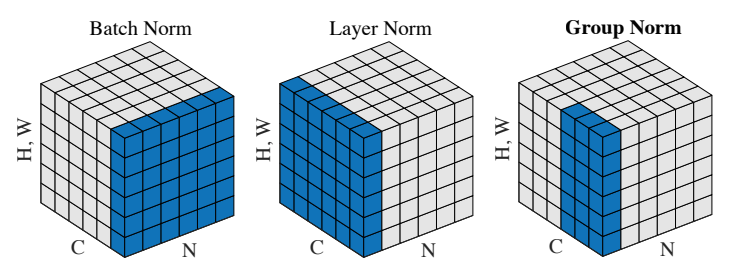
\includegraphics[width=.7\textwidth]{normalization.png}
	\caption{Visual comparison of the normalization techniques discussed so far}
	\label{fig:norm}
\end{figure}

To implement group normalization, we have to take good care of the dimensions but the basic idea is still similar to batch normalization:

\begin{lstlisting}
N, C, H, W = x.shape
x = x.reshape((N, G, -1))
mu = np.mean(x, 2, keepdims=True)
var = np.std(x, 2, keepdims=True)
var_inv = 1 / np.sqrt(var**2 + eps)

x_hat = (x - mu) * var_inv
x_hat = x_hat.reshape((N, C, H, W))
x = x.reshape((N, C, H, W))
out = gamma * x_hat + beta
\end{lstlisting}

We can perform backward pass with the similar idea:
\begin{lstlisting}
N, C, H, W = dout.shape
grouped_shape = (N, G, -1)
m = C//G * H * W

dgamma = np.sum(x_hat * dout, axis=(0, 2, 3), keepdims=True)
dbeta = np.sum(dout, axis=(0, 2, 3), keepdims=True)

dx_hat = dout * gamma
dx_hat = dx_hat.reshape(grouped_shape)
x_hat = x_hat.reshape(grouped_shape)
dx = var_inv / m * \
(dx_hat * m - dx_hat.sum(2, keepdims=True) - x_hat * np.sum(dx_hat * x_hat, axis=2, keepdims=True))
dx = dx.reshape((N, C, H, W))
\end{lstlisting}

\subsection{Training Convolutional Network with PyTorch}
Assignment 2 requires us to implement convnet with PyTorch on different levels of abstractions, which will help us to understand it better.

\paragraph{Barebones PyTorch}
In this part we should use basic PyTorch functions to implement a three-layered convolutional network of two conv layers with ReLU activation and a fully-connected layer, where torch.nn.functional.relu serves as ReLU nonlinearity, torch.nn.functional.conv2d as conv layers, and matrix multiplication as FC layer. Functions in torch.nn.functional need specific data and weighted parameters as the input, which means the abstraction level and convenience are low but flexibility is high. The gradients can be automatically computed by PyTorch with the autograd feature, which is quite awesome, but we have to manually update the parameters.

\paragraph{PyTorch Module API}
Barebone PyTorch requires that we track all the parameter tensors by hand. This is fine for small networks with a few tensors, but it would be extremely inconvenient and error-prone to track tens or hundreds of tensors in larger networks. PyTorch provides the nn.Module API for users to define arbitrary network architectures, while tracking every learnable parameters for us. In the previous part, we implemented SGD ourselves. PyTorch also provides the torch.optim package that implements all the common optimizers, such as RMSProp, Adagrad, and Adam. For example, we can define a convolutional layer using torch.nn.Conv2d fed with parameters that define the shape of the conv layer such as the input channels, filter numbers and filter shapes, but input data are not needed and weights are wrapped up inside the module. PyTorch module API provides higher abstraction and convenience than barebones PyTorch, but less flexibility.

\paragraph{PyTorch Sequential API}
For simple models like a stack of feed forward layers, we still need to go through 3 steps: subclass nn.Module, assign layers to class attributes in \_\_init\_\_, and call each layer one by one in forward(). PyTorch provides a container Module called nn.Sequential, which merges the above steps into one. It is not as flexible as nn.Module, because you cannot specify more complex topology than a feed-forward stack, but it's good enough for many use cases.

In the final part of the assignment we are asked to train a model with whatever ConvNet architecture on CIFAR-10 and achieve at least 70\% accuracy on the CIFAR-10 validation set within 10 epochs.

The default setting(3-layered convnet) achieves 50\% accuracy, so there is a long way to go. First I random search learning rate to find the optimal result. It turns out that setting learning rate to be 1.8e-3 will increase the accuracy to be 59.8\%. Then I insert batch normalization layers after each conv layer and stack more conv layers(6 conv layers in total), and all kernels have size $3\times 3$. At the same time I set every two conv layers striding 2 instead of 1 to perform as dropout. The final 7-layered convnet trained in 10 epochs easily achieves 74.86\% accuracy on validation set, outperforming the baseline by 4.86\%. The model also has 74.8\% accuracy on test set, showing that there is little overfitting problem.

\section{Plans}
In the next I will try to re-implement convnet exercise with TensorFlow since the TensorFlow exercise is also provided by the assignment 2 of cs231n course. And also I will continue the course.

\end{document}
